
\documentclass[11pt, a4paper]{article}


%%%%%%%%%% Import Packages %%%%%%%%%

\usepackage[margin=2cm]{geometry} % 2cm margins
\usepackage{amsmath,amsthm,amssymb} % AMS math environment
\usepackage{bm}         % bold in math mode
\usepackage{fontspec}   % font setting
\usepackage{type1cm}    % fontsize setting
\usepackage{titlesec}   % section, subsection ... font setting
\usepackage{titling}    % title setting
\usepackage{fancyhdr}   % header and footer
\usepackage{enumerate}  % improving enumerate
\usepackage{stmaryrd}   % some math fonts
\usepackage[square, comma, numbers, sort&compress]{natbib} % bibliography
\usepackage[usenames, dvipsnames]{color} % to use colors
\usepackage{hyperref}   % advanced reference
\usepackage{multicol}   % separte reference in two columns

%%%%%%%%%%% For figures %%%%%%%%%%
\usepackage{graphicx}    % insert figures
\usepackage{float}

%%%%%%%%%% Table and caption packages %%%%%%%%%%%
\usepackage{booktabs} % toprule, bottomrule ...
\usepackage{tabu}
\usepackage{multirow}
\usepackage{tabularx}
\usepackage{caption}
\usepackage{caption3}
\usepackage{subcaption}

%%%%%%%%%% Chinese Environment %%%%%%%%%%
\usepackage[AutoFakeBold, CheckSingle, CJKmath]{xeCJK}  % xelatex Chinese
\usepackage{CJKulem}	% Chinese character decoration


%%%%%%%%%% Page settings %%%%%%%%%% 
\setlength{\headheight}{15pt}  % with titling
\setlength{\droptitle}{-1.5cm} % white space before the title
\setlength{\bibsep}{1.2ex} % bibliography vertical spacing
\parindent=0pt % indent spacing
\parskip=0.8em  % spacing between two paragraphs


%%%%%%%%%% Math display spacing (gather, equation, ...) %%%%%%%%%%
\makeatletter
\g@addto@macro\normalsize{%
  \setlength{\abovedisplayskip}{-8pt}
  \setlength{\belowdisplayskip}{4pt}
  \setlength{\abovedisplayshortskip}{-8pt}
  \setlength{\belowdisplayshortskip}{4pt}
}


%%%%%%%%%% Figure caption %%%%%%%%%%
\captionsetup[figure]{%
 	font = small,
	name = \textbf{Figure},
	justification = justified, % caption as normal paragraph
    labelsep = colon, % Figure: ...
	skip = 1.1em} % space between caption and image
\captionsetup[sub]{font = small, belowskip = 2pt}
\setlength{\belowcaptionskip}{-15pt}
\setlength{\intextsep}{20pt}


%%%%%%%%%% Figure position %%%%%%%%%%
\graphicspath{%
{../figures/},
}


%%%%%%%%%% Table settings %%%%%%%%%%
\captionsetup[table]{%
  parskip = 20pt,
  font = small,
  name = \textbf{Table},
  justification = justified,
  belowskip=7pt,
  skip = \medskipamount,
  singlelinecheck = false
}
\renewcommand{\arraystretch}{1.2}
\tabcolsep = 10pt


%%%%%%%%%% Reference settings %%%%%%%%%%
\hypersetup{%
unicode=true, 
bookmarksdepth=-1, 
pdfborder={0 0 0}, 
colorlinks=true, 
linkcolor=RoyalBlue,
citecolor=blue
}


%%%%%%%%%% Seperate reference in two columns %%%%%%%%%%
\makeatletter
\renewenvironment{thebibliography}[1]
     {\begin{multicols}{2}[\section*{\refname}]%
      \@mkboth{\MakeUppercase\refname}{\MakeUppercase\refname}%
      \list{\@biblabel{\@arabic\c@enumiv}}%
           {\settowidth\labelwidth{\@biblabel{#1}}%
            \leftmargin\labelwidth
            \advance\leftmargin\labelsep
            \@openbib@code
            \usecounter{enumiv}%
            \let\p@enumiv\@empty
            \renewcommand\theenumiv{\@arabic\c@enumiv}}%
      \sloppy
      \clubpenalty4000
      \@clubpenalty \clubpenalty
      \widowpenalty4000%
      \sfcode`\.\@m}
     {\def\@noitemerr
       {\@latex@warning{Empty `thebibliography' environment}}%
      \endlist\end{multicols}}
\makeatother

\begin{document}

%mainfile: Multimodal_learning.tex

\title{Multimodal Learning: Examples in Gesture and Audio-Visual
Speech Recognition\vspace{-0.5em}}
\author{Hsieh Yu-Guan}
\date{\today}
\maketitle

\section*{Abstract}

\section{Introduction}

\section{Related Work}

\section{Presentation of Basic Network Architectures}

\section{Datasets and Preprocessing}

Many datasets were explored during my internship. The three main datasets
being used are given in details  below. Two of them are for gesture
recognition:
Creative Senz3D \cite{A. Memo 2015, A. Memo 2017} and ASL Finger Spelling
\cite{N. Pugeault 2011}, and one is for AVSR: AVLetters
\cite{I. Matthews 2002}.

\subsection{Creative Senz3D}

The dataset contains gestures perfomed by 4 different people, each
performing 11 different static gestures repeated 30 times each,
for a total of 1320 samples.
For each sample, color, depth and confidence frames are available.
I only used the color and depth frames of this dataset. The original
size of each image is $480 \times 640$ and they're resized to
$299 \times 299$ pixels before being fed to the network. No other
preprocessing are done. For both color and depth images I use the three
color channels (even though a priori only one channel is needed for
depth maps).

\begin{figure}[H]
  \centering
  \hfill
  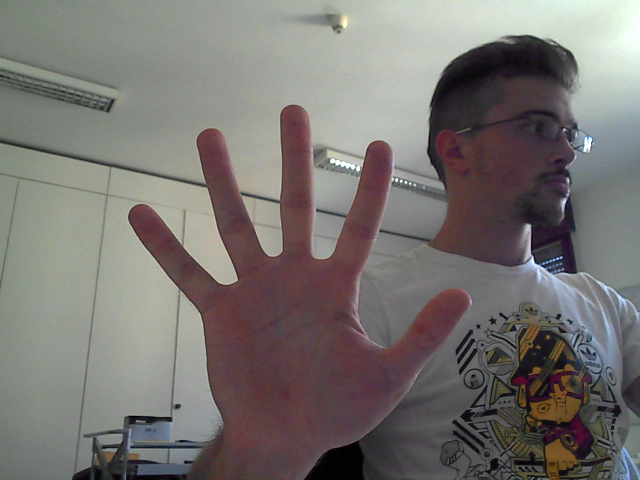
\includegraphics[width=0.23\linewidth]{dataset/senz3d/examples/1-color}
  \hfill
  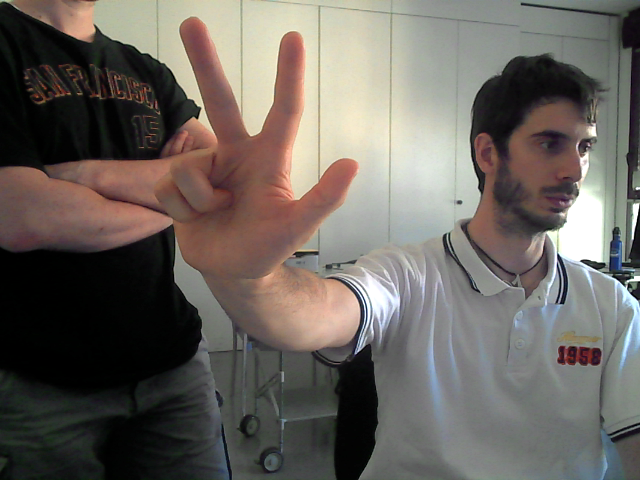
\includegraphics[width=0.23\linewidth]{dataset/senz3d/examples/12-color}
  \hfill
  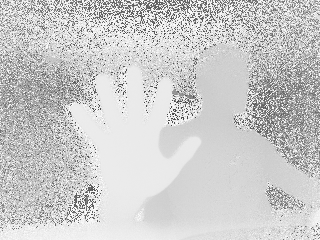
\includegraphics[width=0.23\linewidth]{dataset/senz3d/examples/1-depth}
  \hfill
  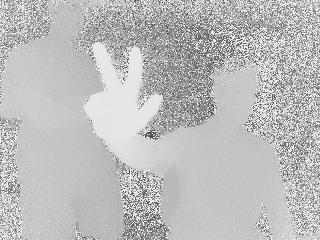
\includegraphics[width=0.23\linewidth]{dataset/senz3d/examples/12-depth}
  \caption{%
    \textbf{Example images in the Creative Senz3D dataset.}\\[0.1em]
    Left Two) Color images.\\[0.1em]
    Right Two) Corresponding depth images.\\[0.1em]
    All of the images are of size $480 \times 640$ and contain the
      the entire upper body of the subject.}
  \label{fig:senz3d_exs}
\end{figure}

\subsection{ASL Finger Spelling}

The dataset is composed of more than 60000 images in each modality
(RGB and depth images are provided).
Five subjects are asked to perform the 24 static signs in
the American Sign Language (ASL) alphabet (excluding j and z which involve
motion) a certain number of times, captured with similar lighting
and background.

Images of this dataset are of variable sizes. The data preprocessing
includes resizing each image to $83 \times 83$ pixels,
converting to grayscale and adjusting
contrast of depth maps. Only very late in my internship I added the
Z-normalization (normalize to zero mean and unit of variance)
as a preprocessing step and the only result that was largely changed
is presented in \ref{subsection:CAE}.

\begin{figure}[H]
  \centering
  \hfill
  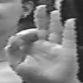
\includegraphics[width=0.15\linewidth]{%
    dataset/fingerspelling5/exs/or/g1}
  \hfill
  
\includegraphics[width=0.15\linewidth]{%
    dataset/fingerspelling5/exs/or/g2}
  \hfill
  
\includegraphics[width=0.15\linewidth]{%
    dataset/fingerspelling5/exs/or/d3}
  \hfill
  
\includegraphics[width=0.15\linewidth]{%
    dataset/fingerspelling5/exs/or/d4}
  \hfill
  
\includegraphics[width=0.15\linewidth]{%
    dataset/fingerspelling5/exs/st/d1}
  \hfill
  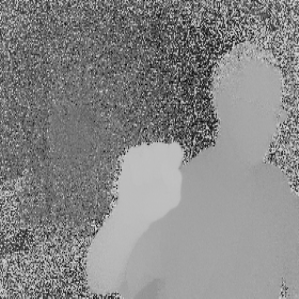
\includegraphics[width=0.15\linewidth]{%
    dataset/fingerspelling5/exs/st/d2}
  \caption{%
    \textbf{Example images in the ASL Finger Spelling dataset
      (after preprocessing).}\\[0.1em]
    Left Two) Grayscale intensity images.\\[0.1em]
    Middle Two) Depth maps after adjusting contrast.\\[0.1em]
    Right Two) Depth maps after Z-normalization.\\[0.1em]
    Images of this dataset have variable sizes, and they're all resized to
      $83 \times 83$ before being fed to the network. Generally only the
      hand region is contained in image.}
  \label{fig:fingerspelling_exs}
\end{figure}

\subsection{AVLetters}

The dataset comprises video and audio recordings of 10 speakers
uttering the letters A to Z, three times each.
We count therefore 780 samples in total. For video data, image sequences
of pre-extracted lip regions are provided.
Each single image if of size $60 \times 80$.
For audio data, only the mel-frequency cepstrum coefficients (MFCCs)
are given, and each audio frame is represented by 26 mfccs.
The lack of raw audio data is a strong constraint on what we're able to do
on this dataset.

Since all utterances don't have the same time duration, I used
fourier resamping to force every video input to be of length 12 and
every audio input to be of length 24. Video frames are Z-normalized.
Several data augmentation techniques
are also considered, including random brightness adjusting, random contrast
adjusting and random cropping (but at least 80\% of the original image
is kept).

\begin{figure}[H]
  \centering
  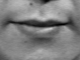
\includegraphics[width=0.15\linewidth]{%
    dataset/avletters/lips_no_data_aug/1}
  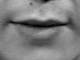
\includegraphics[width=0.15\linewidth]{%
    dataset/avletters/lips_no_data_aug/2}
  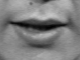
\includegraphics[width=0.15\linewidth]{%
    dataset/avletters/lips_no_data_aug/3}
  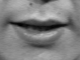
\includegraphics[width=0.15\linewidth]{%
    dataset/avletters/lips_no_data_aug/4}
  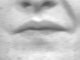
\includegraphics[width=0.15\linewidth]{%
    dataset/avletters/lips_no_data_aug/5}
  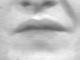
\includegraphics[width=0.15\linewidth]{%
    dataset/avletters/lips_no_data_aug/6}\\[0.15em]
  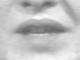
\includegraphics[width=0.15\linewidth]{%
    dataset/avletters/lips_no_data_aug/7}
  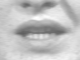
\includegraphics[width=0.15\linewidth]{%
    dataset/avletters/lips_no_data_aug/8}
  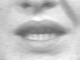
\includegraphics[width=0.15\linewidth]{%
    dataset/avletters/lips_no_data_aug/9}
  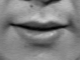
\includegraphics[width=0.15\linewidth]{%
    dataset/avletters/lips_no_data_aug/10}
  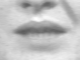
\includegraphics[width=0.15\linewidth]{%
    dataset/avletters/lips_no_data_aug/11}
  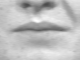
\includegraphics[width=0.15\linewidth]{%
    dataset/avletters/lips_no_data_aug/12}
  \caption{%
    \textbf{Example visual input for the AVletters dataset
      (left to right, top to bottom).}\\[0.1em]
    Pre-extracted lip regions of $60 \times 80$ pixels are provided.
      Each image sequence is resampled to be of length twelve in order to
      give an input of fixed size to the network.}
  \label{fig:avletters_exs}
\end{figure}

\section{Experimental Setup}

\section{Experiences and Results: Unimodal Cases}

\subsection{Classification}

With every new dataset, I began with training a classifier on it in a
totoally supervised manner.
This gave me an insight into its data quality, the preprocessing
effectiveness and ensured that further experiments could be conducted.
CNN is then one of the most suitable architecture for this purpose.

\subsubsection{Creative Senz3d}

No satisfying results were acquired. It may be due to to a lack of data
quantity, variety, and the fact that the head is also contained in the
image increases significantly the classification difficulty.

\textbf{Subject Dependent.}
In a subject dependant setting, images are separated randomly into
training set (3/4) and test set (1/4). Therefore, during the
testing phase, the classifier doesn't need to deal with data from an
individual that it has never seen before.
In this case, for RGB images, all of the classifiers are able to
have a classification accuracy that is closed to 100\%. This holds true
even for a perceptron.
On the other hand, for depth images, the classification accuracy is
between 60\% and 70\% using a perceptron and near 90\% for other CNN
architectures that were tested.

\textbf{Subject Independant.}
On the contrary, the classifier faces individuals never seen before
during testing in a subject independant setting. 
In my case, the training set consists of images coming from the
first three individuals while the test set contains images of
the final subject.
With the various architectures (including single-layer perceptron
and CNNs varying from three to ten hidden layers)
that I implemented, none of them is able to generalize the learned model
to the new individual.
The pre-trained InceptionV4 architecture achieves a prediction accuracy
of 30\% for color images and 20\% for depth images (better than chance).

\subsubsection{ASL Finger Spelling}

The large number of data contained in this dataset and the relatively
simple image content (single hand instead of the entire upper body)
makes the classification task much easier. By using the CNN architecture
shown in \autoref{fig:CNN10}, we can achieve a classification accuracy
of respectively 80\% and 70\% for intensity and depth images (Table 1)
in an subject-independant setting (four subjects for training and one
subject for testing). We may not need that many layers in the CNN
architecture, but further tests were not carried out since it's not
the essential point of my internship.

\begin{figure}[H]
  \centering
  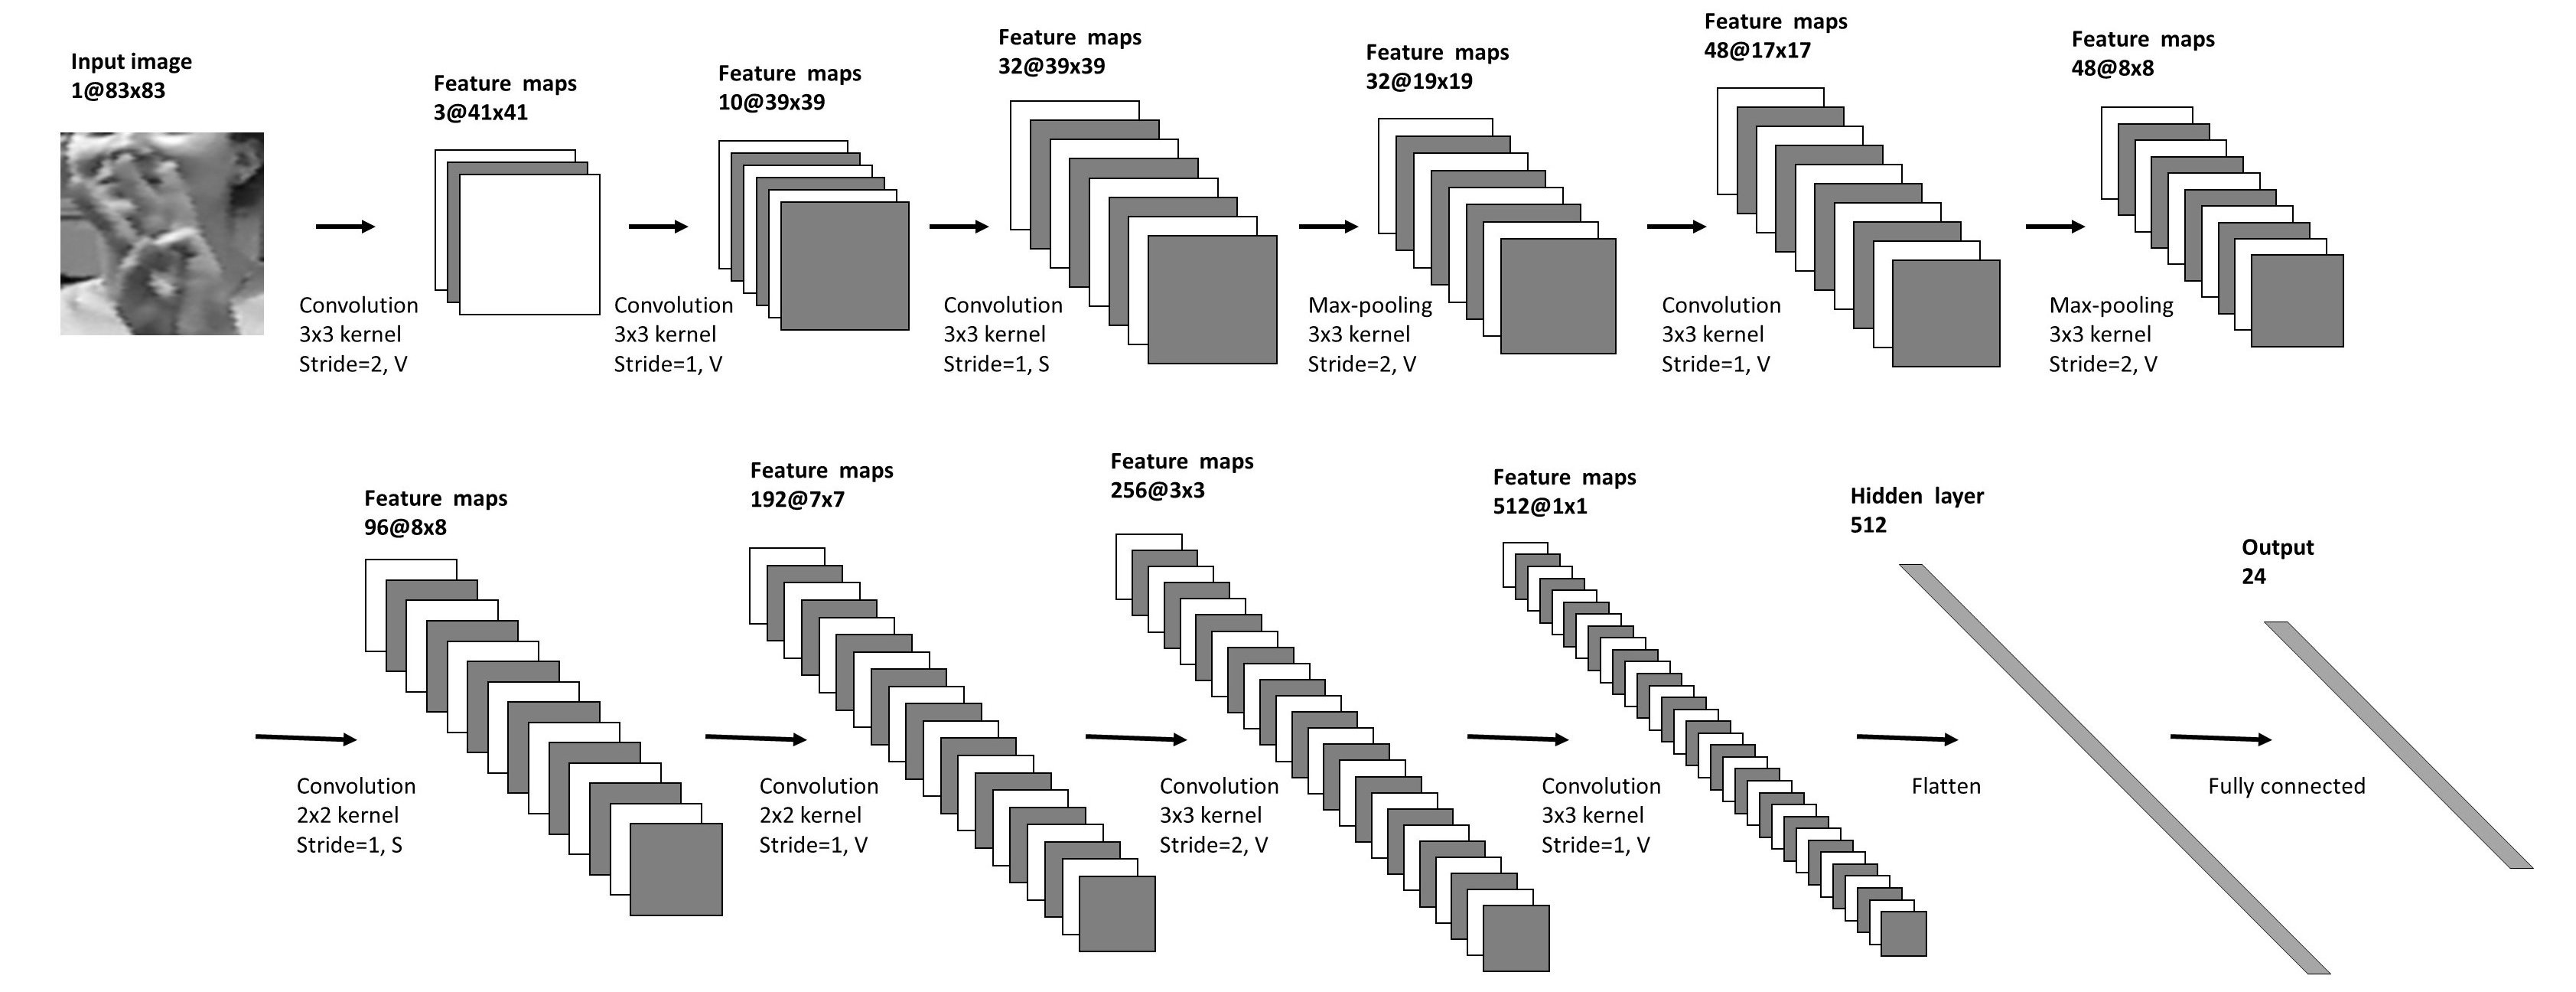
\includegraphics[width=\linewidth]{architectures/CNN10}
  \caption{%
    \textbf{CNN architecture used for the Finger Spelling  dataset.}
      \\[0.1em]
    The input of the nework is a one-channel image of size $83 \times 83$.
      It contains ten hidden layers. S stands for `SAME' padding
      and V stands for `VALID' padding (see text).}
  \label{fig:CNN10}
\end{figure}

\subsubsection{AVletters}

One can refer to \autoref{fig:AVSR_transfer} for the main CNN architectures
that are used in this dataset. 
Notice that 3d CNNs are employed to deal with video inputs.
Considering the small number of available data, a speaker-dependant
setting was used, but it didn't save me from the problem of overfitting.
The classification accuracy is of 100\% for training data but only
of 60\% or 55\% for testing data depending on the input modality
(audio then video).

Curiously, for audio data, I get exactly the same classification
performance regardless of the used architecture (perceptron or CNNs)
or the fact that if deltas and delta-deltas are also given in input.
This is not the case when I test with another audio dataset
(not mentioned in the Datasets and Preprocessing section beacause
it wasn't used for main experiences).
For video input, the use of data augmentation techniques only decrease
the learning speed for the training part but doesn't improve the performace
for testing.

\subsection{Convolutional auto-encoder} \label{subsection:CAE}

\begin{figure}[H]
  \centering
  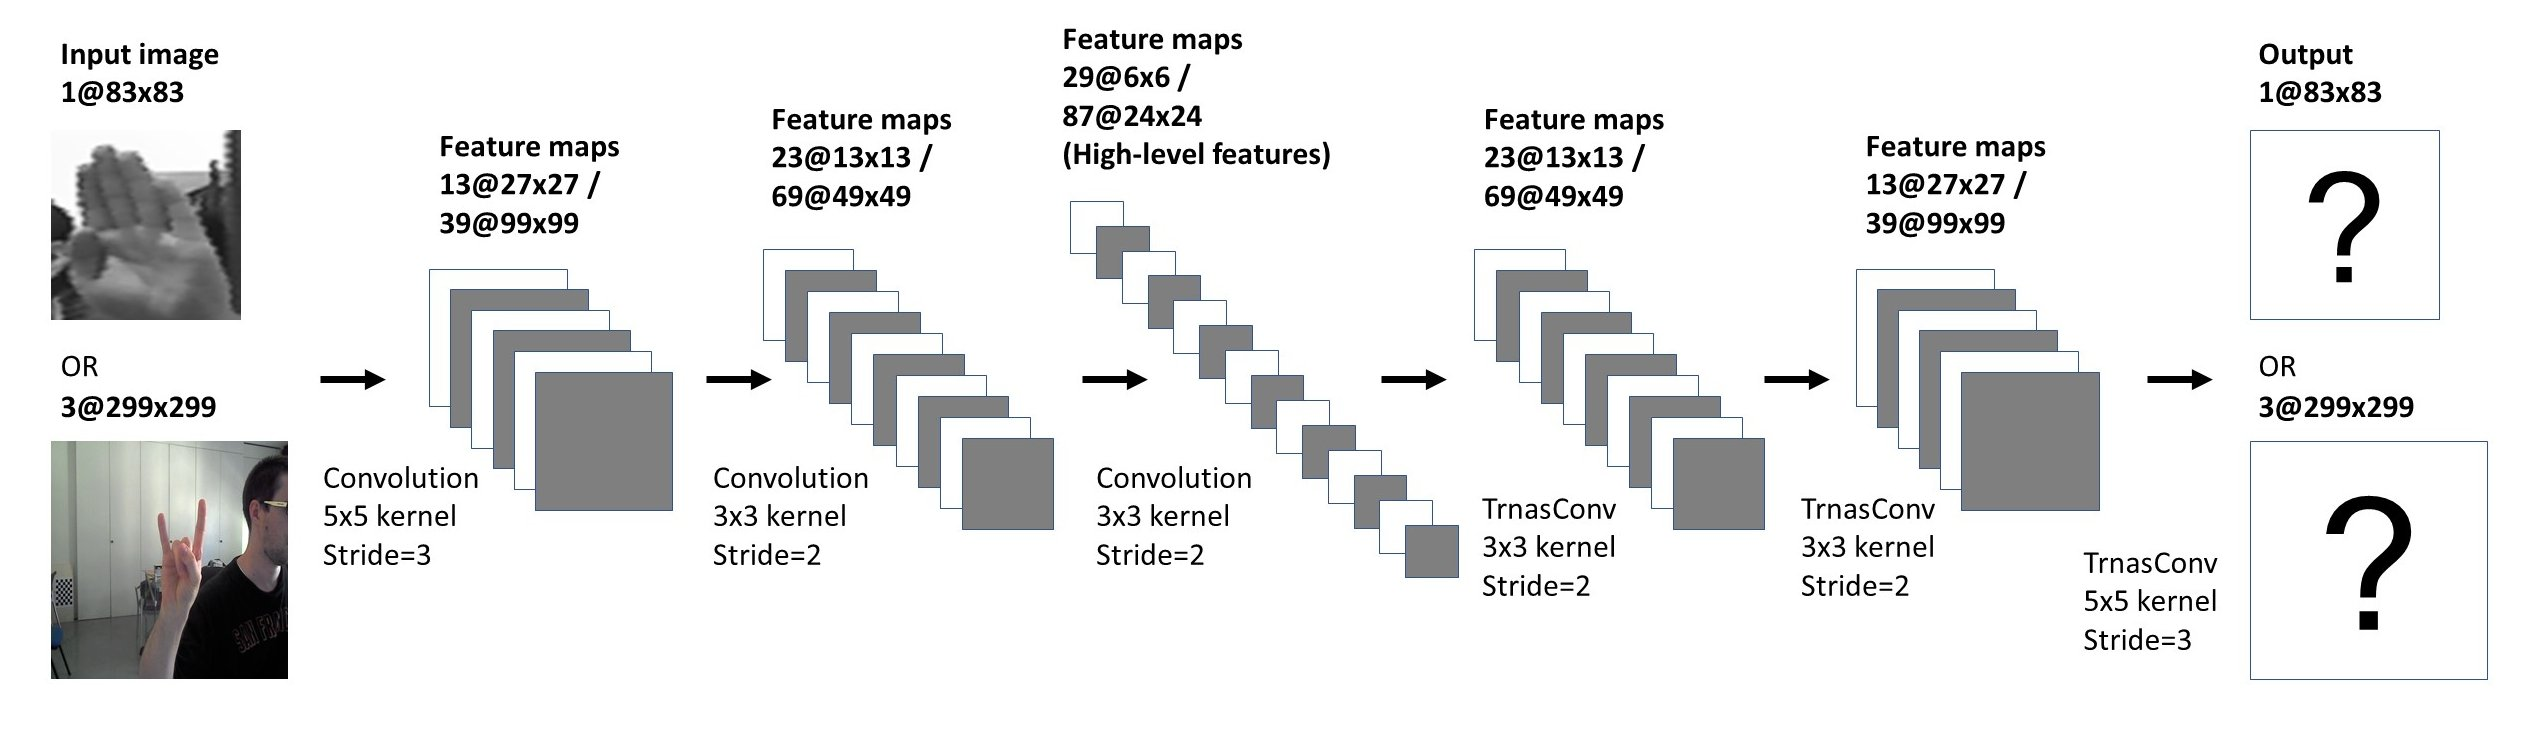
\includegraphics[width=\linewidth]{architectures/CAE5}
  \caption{%
    \textbf{Convolutional auto-encoder architecture with 
      three convolutional layers and three tranposed convolutional
      layer.}\\[0.1em]
    Activation values of the middle layer are taken as 
      high-level features of the input image. Inputs of the network
      can be of different sizes. We only use valid paddings here.}
  \label{fig:CAE5}
\end{figure}

\begin{figure}[H]
  \centering
  \hfill
  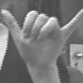
\includegraphics[width=0.28\linewidth]{%
    dataset/fingerspelling5/gray/gray4}
  \hfill
  
\includegraphics[width=0.28\linewidth]{%
    dataset/fingerspelling5/gray/gray_dropout4}
  \hfill
  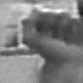
\includegraphics[width=0.28\linewidth]{%
    dataset/fingerspelling5/gray/gray_reconstruction4}
  \caption{%
    \textbf{Image restoration using convolutional auto-encoder.}\\[0.1em]
      Left) Clean Image.\\[0.1em]
      Middle) Noisy image [input].\\[0.1em]
      Right) Restored image [output].}
  \label{fig:image_restoration}
\end{figure}

\section{Experiences and Results: Multimodal Cases}

\subsection{Learning shared representation}

\begin{figure}[H]
  \centering
  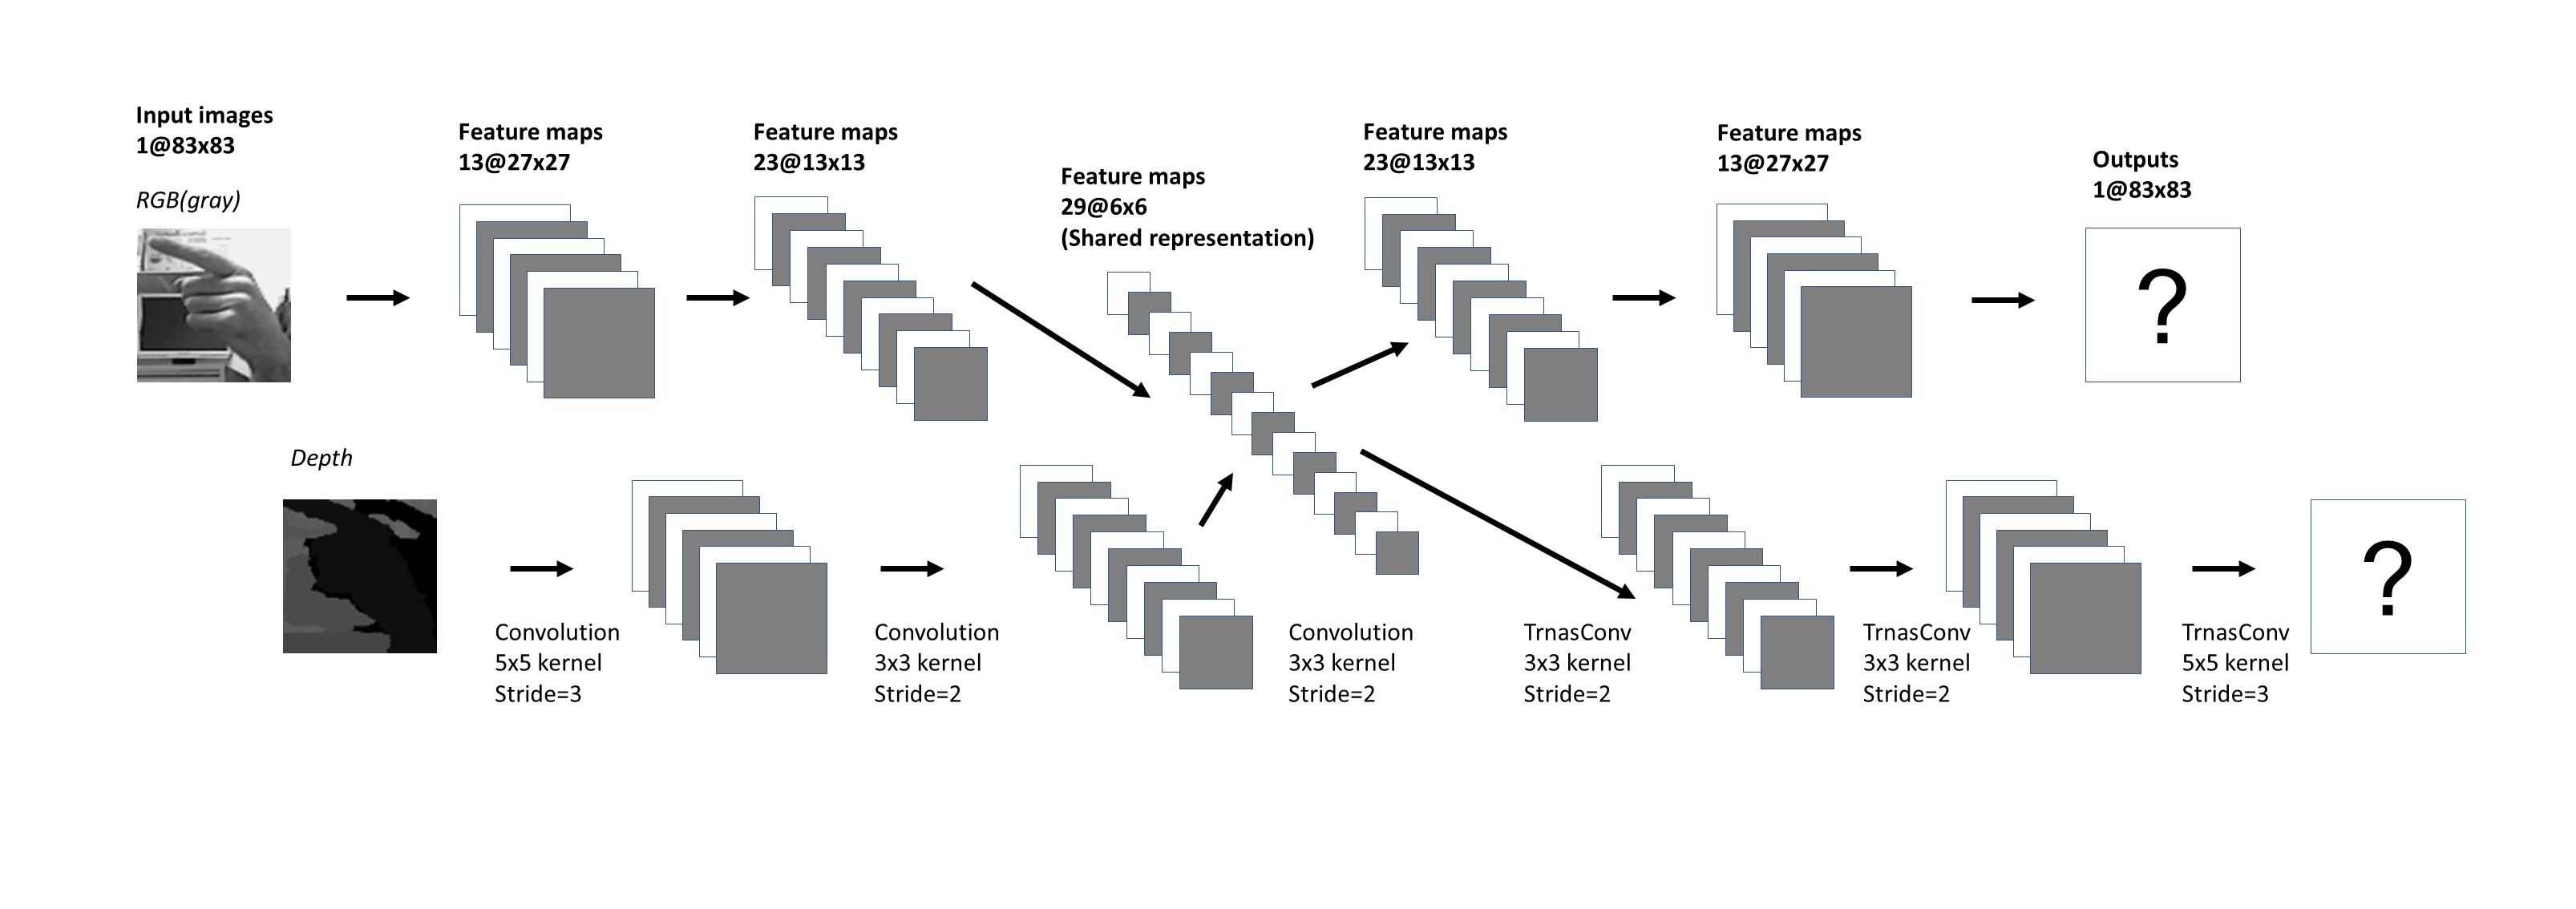
\includegraphics[width=\linewidth]{architectures/FAE5}
  \caption{%
    \textbf{The bimodal convolutional auto-encoder model that is
      used to learn shared multimodal representation.}\\[0.1em]
    We simply take the CAE architecture that is introduced earlier
      (\autoref{fig:CAE5}) for each modaliy but force them to have a
      shared middle layer by adding the corresponding activation values.
      We then try to reconstruct the two images separately through
      two disjoint paths.}
  \label{fig:FAE5}
\end{figure}

\begin{figure}[H]
  \centering
  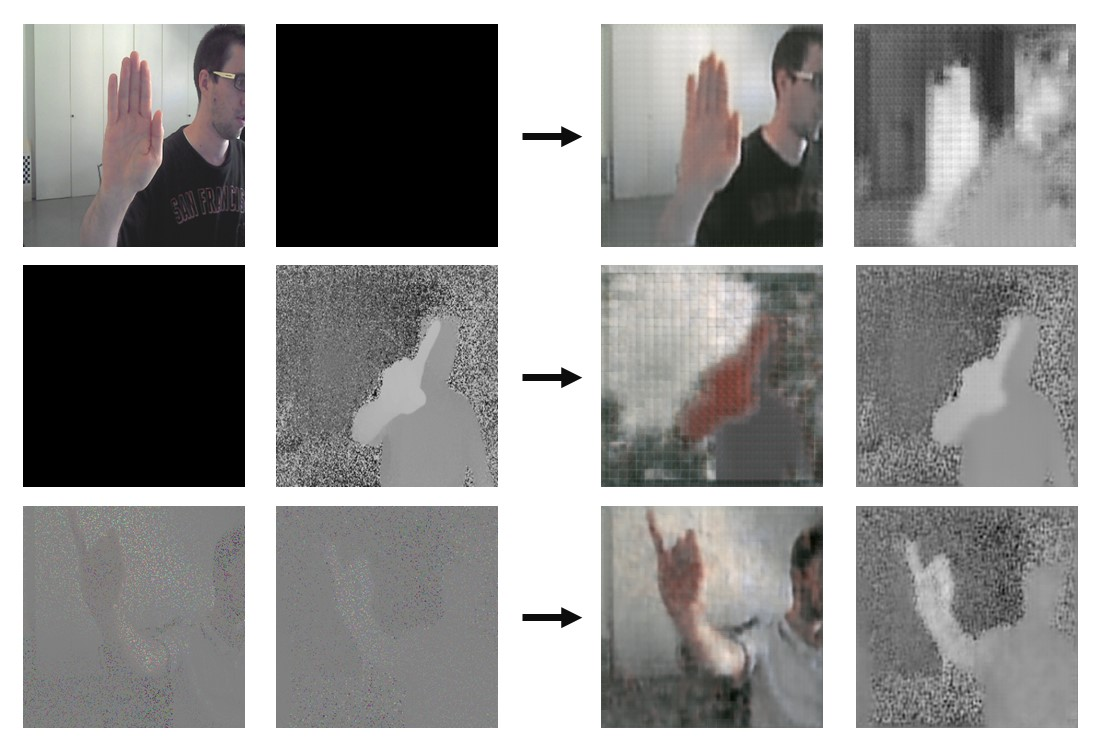
\includegraphics[width=\linewidth]{dataset/senz3d/reconstructions}\\[-1em]
  \caption{%
    \textbf{Restore color and depth images from incomplete input
      information.}\\[0.1em]
    Top) Only the color image is given.\\[0.1em]
    Middle) Only the depth image is given.\\[0.1em]
    Botttom) Both modalities are given but with little information
      (10\% of pixels).}
  \label{fig:color_depth_restoration}
\end{figure}

\subsection{Transfer learning}

\begin{figure}[H]
  \centering
  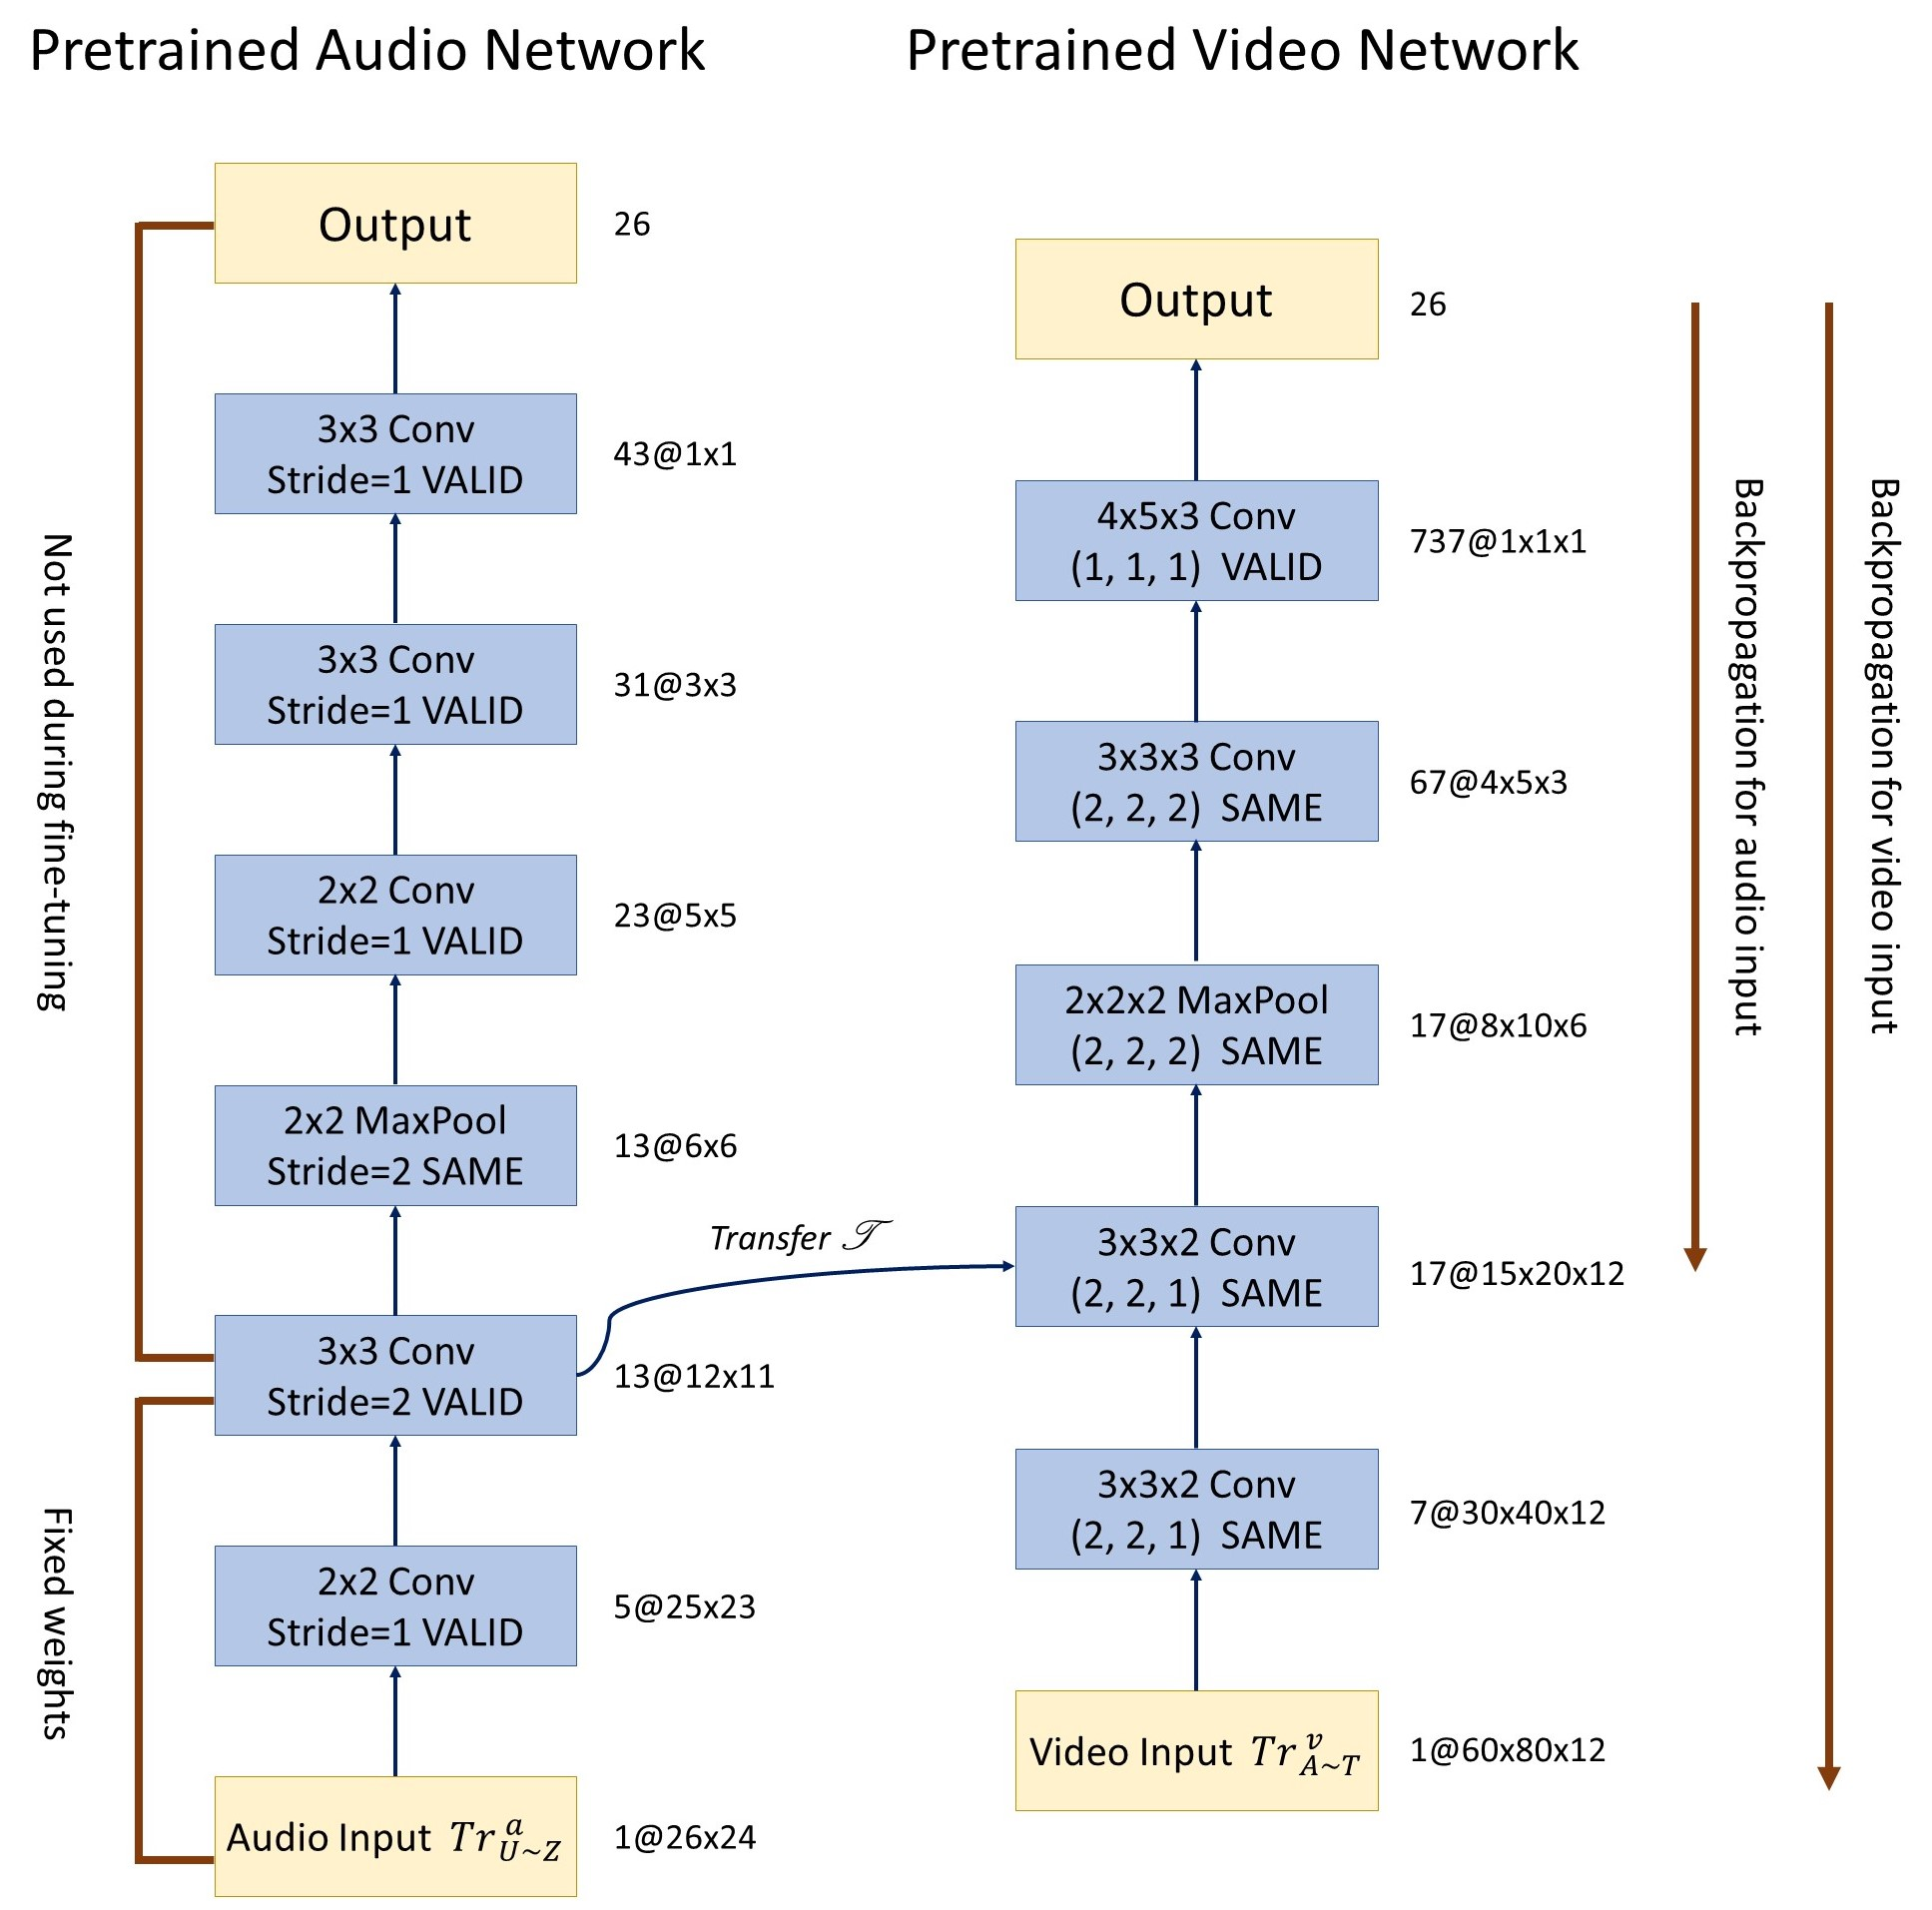
\includegraphics[width=0.9\linewidth]{architectures/AVSR_transfer}\\[-1em]
  \caption{%
    \textbf{Illustration of the transfer learning approach applied in
      audio and lip-reading speech recognition tasks.}\\[0.1em]
    We first learn two separated model for audio and visual inputs
      (in my cases two CNNs) and try to fine-tune the video network
      with transferred audio data.
    }
  \label{fig:AVSR_transfer}
\end{figure}

\newpage

\begin{thebibliography}{99}

\bibitem{M. Asadi-Aghbolaghi 2017}
  17. M. Asadi-Aghbolaghi, A. Clapés, M. Bellantonio, H. J. Escalante, 
  V. Ponce-López, X. Baró, I. Guyon, S. Kasaei, and S. Escalera. 
  A Survey on Deep Learning Based Approaches for Action and Gesture 
  Recognition in Image Sequences. 
  In \textit{Automatic Face \& Gesture Recognition (FG 2017) 2017 12th IEEE
  International Conference}, 2017.

\bibitem{T. Baltrusaitis 2017}
  T. Baltrusaitis, C. Ahuja and L-P. Morency. Multimodal Machine Learning:
  A Survey and Taxonomy. In \textit{CoRR}, vol. abs/1705.09406, 2017.

\bibitem{C. Bregler 1994}
  C. Bregler and Y. Konig. "Eigenlips" for robust speech recognition.
  In \textit{ICASSP}, 1994.

\bibitem{L. Deng 2013}
  L. Deng, G. Hinto and B. Kinsbury. New types of deep neural network
  learning for speech recognition and related applications: An overview.
  In \textit{ICASSP}, 2013.

\bibitem{A. Droniou 2014}
  A. Droniou, S. Ivaldi, and O. Sigaud. A deep unsupervised network
  for multimodal perception, representation and classification. In
  \textit{Robotics and Autonomous System}, 2014.

\bibitem{A. Frome 2013}
  A. Frome, G. S. Corrado, J. Shlens, S. Bengio, J. Dean,
  T. Mikolov, et al. Devise: A deep visual-semantic embedding model. 
  In \textit{NIPS}, 2013.

\bibitem{G. Hinton 2012}
  G. Hinton, L. Deng, D. Yu, G. Dahl, A. Mohamed, N. Jaitly, A. Senior, V.
  Vanhoucke, P. Nguyen, T. Sainath and B. Kingsbury. Deep neural networks
  for acoustic modeling in speech recognition.
  In \textit{IEEE Signal Processing Mag} Vol. 29, 2012.

\bibitem{S. Ioffe 2015}
  S. Ioffe and C. Szegedy. Batch normalization, accelerating deep network
  training by reducing internal covaraiate shift. In \textit{CoRR},
  vol. abs/1502.03167, 2015.

\bibitem{S. Ji 2013}
  S. Ji, W. Xu, M Tang and K. Yu. 3D Convolutional Neural Networks
  for Human Action Recognition. In \textit{IEEE Transactions on Pattern
  Analysis and Machine Intelligence}, vol. 35, 2013.

\bibitem{A. K. Katsuaggelos 2015}
  A. K. Katsaggelos, S. Bahaadini and R. Molina. Audiovisual fusion:
  Challenges and new approaches. In \textit{Proceedings of the IEEE},
  vol. 103, 2015.

\bibitem{A. Krizhevsky 2012}
  A. Krizhevsky, I. Sutskever, and G. E. Hinton.  ImageNet Classification
  with Deep Convolutional Neural Networks. In \textit{NIPS}, 2012.

\bibitem{J. Masci 2011}
  J. Masci, U. Meier, D. C. ̧san, and J. Schmidhuber.
  Stacked convolutional auto-encoders for hierarchical feature extraction.
  In \textit{Artificial Neural Networks and Machine Learning–ICANN}, 2011.

\bibitem{I. Matthews 2002}
  I. Matthews, T. F. Cootes, J. A. Bangham and S. Cox. Extraction of visual
  features for lipreading. In \textit{PAMI}, 2002.

\bibitem{A. Memo 2015}
  A. Memo, L. Minto and P. Zanuttigh.  Exploiting Silhouette Descriptors and
  Synthetic Data for Hand Gesture Recognition. In \textit{STAG: Smart
    Tools \& Apps for Graphics}, 2015.

\bibitem{A. Memo 2017}
  A. Memo and P. Zanuttigh. Head-mounted gesture controlled interface
  for human-computer interaction. In \textit{Multimedia Tools and
  Applications}, 2017.

\bibitem{S. Mitra 2007}
  S. Mitra and T. Acharya. Gesture recognition: A survey. 
  In \textit{IEEE Systems, Man, and Cybernetics}, 37:311–324, 2007. 

\bibitem{P. Molchanov 2015}
  P. Molchanov, S. Gupta, K. Kim, and J. Kautz. Hand gesture recognition 
  with 3D convolutional neural networks. In \textit{CVPRW}, 2015.

\bibitem{S. Moon 2015}
  S. Moon, S. Kim and H. Wang. Multimodal transfer deep learning with
    applications in audio-visual recognition. In \textit{NIPS MMML
    Workshop}, 2015.

\bibitem{J. Nagi 2011}
  J. Nagi, F. Ducatelle, G. Di Caro, D. Ciresan, U. Meier, A. Giusti,
  F. Nagi, J. Schmidhuber, and L. Gambardella.
  Max-pooling convolutional neural networks for vision-based hand 
  gesture recognition.
  In \textit{Proceedings of the IEEE International Conference on
  Signal and Image Processing Applications}, 2011.

\bibitem{N. Neverova 2014}
  N. Neverova, C. Wolf, G. W. Taylor, and F. Nebout.  Multiscale deep
  learning for gesture detection and localization. In \textit{ECCVW}, 2014.

\bibitem{J. Ngiam 2011}
  J. Ngiam, A. Khosla, M. Kim, J. Nam, and A. Y. Ng. 
  Multimodal deep learning. In:
  In \textit{International Conference on Machine Learning}.  28. 
  Bellevue, Washington, USA, 2011.

\bibitem{K. Noda 2014}
  K. Noda, Y. Yamaguchi, K. Nakadai, H. G. Okuno and T. Ogata. Audio-visual
  speech recognition using deep learning.  In \textit{Applied Intelligence,
  vol. 42, no. 4, pp. 722–737, 2014.}

\bibitem{E. Petahan 1988}
  E. Petahan, B. Bischoff, D. Bodoff, and N. M. Brooke. An Improved
  Automatic Lipreading System to enhance Speech Recognition.
  In \textit{ACM SIGCHI}, 1988.

\bibitem{L. Pigou 2014}
 L. Pigou, S. Dieleman, P. J. Kindermans, and B. Schrauwen.
  Sign language recognition using convolutional neural networks. In
  \textit{Workshop at the European Conference on Computer Vision},
  pages 572--578, 2014.

\bibitem{G. Potamianos 2004}
  G. Potamianos, C. Neti, J. Luettin and  I. Matthews. Audio-visual
  automatic speech recognition: An overview. In \textit{Issues in Visual
  and Audio-Visual Speech Processing, MIT Press}, 2004.

\bibitem{N. Pugeault 2011}
  N. Pugeault, and R. Bowden. Spelling It Out: Real-Time ASL
  Fingerspelling Recognition. In \textit{Proceedings of the 1st IEEE
  Workshop on Consumer Depth Cameras for Computer Vision}, 2011.

\bibitem{R. Socher 2013}
  R. Socher, M. Ganjoo, H. Sridhar, O.Bastani, C. D. Manning, and
  A. Y. Ng. Zero-shot learning through cross-modal transfer.
  In \textit{International Conference on Learning Representations (ICLR)},
  Scottsdale, Arizona, USA, 2013.

\bibitem{N. Srivastava 2014}
  N. Srivastava, G. Hinton, A. Krizhevsky, I. Sutskever and R. Salakhutdinov.
  Dropout: A simple way to prevent neural networks from overfitting. In
  \textit{Journal of Machine Learning Research}, vol. 15, 2014.

\bibitem{T. Starner 1998}
  T. Starner, A. Pentland, and J. Weaver. Real-time american sign language
  recognition using desk and wearable computer based video. 
  In \textit{PAMI}, 20(12):1371–1375, 1998.

\bibitem{J. Sung 2015}
  J. Sung, I. Lenz, and A. Saxena. Deep multimodal embedding:
  Manipulating novel objects with point-clouds, language and trajectories.
  In \textit{CoRR}, vol. abs/1509.07831, 2015.

\bibitem{C. Szegedy 2016}
  C. Szegedy, S. Ioffe, V, Vanhoucke. Inception-v4, inception-ResNet and the
  impact of residual connections on learning. In \textit{CoRR},
  vol. abs/1602.07261, 2016.

\bibitem{V. Turchenko 2017}
  V. Turchenko, E. Chalmers and A. Luczak. A deep convolutional auto-encoder
  with pooling - unpooling layers in Caffe. In \textit{CoRR},
  vol. abs/1701.04949, 2017.

\bibitem{J. Weston 2010}
  J. Weston, S. Bengio, and N. Usunier. 
  Large scale image annotation: learning to rank with joint word-image
  embeddings. In \textit{Machine Learning}, 81(1):21--35, 2010.

\bibitem{Di Wu 2016}
  Di Wu, Lionel Pigou, Pieter-Jan Kindermans, Nam Do-Hoang Le, Ling Shao,
  Joni Dambre, and Jean-Marc Odobez. 
  Deep Dynamic Neural Networks for Multimodal Gesture Segmentation and
  Recognition. In \textit{Pattern Analysis and Machine Intelligence
  IEEE Transactions}, vol. 38, 2016.

\bibitem{B. P. Yuhas 1989}
  B. P. Yuhas, M. H. Goldstein, and T. J. Sejnowski. Integration of acoustic
  and visual speech signals using neuralnetworks. in \textit{IEEE Comm.
  Magazine}, pp. 65--71, 1989.

\end{thebibliography}


%mainfile: Multimodal_learning.tex

\vspace{-0.3em}
\bibliographystyle{abbrv}
\begin{thebibliography}{99}

{\footnotesize

\bibitem{M. Asadi-Aghbolaghi 2017}
  M. Asadi-Aghbolaghi, A. Clapés, M. Bellantonio, H. J. Escalante, 
  V. Ponce-López, X. Baró, I. Guyon, S. Kasaei, and S. Escalera. 
  A Survey on Deep Learning Based Approaches for Action and Gesture 
  Recognition in Image Sequences. 
  In \textit{Automatic Face \& Gesture Recognition (FG 2017) 2017 12th IEEE
  International Conference}, 2017.

\bibitem{T. Baltrusaitis 2017}
  T. Baltrusaitis, C. Ahuja and L-P. Morency. Multimodal Machine Learning:
  A Survey and Taxonomy. In \textit{arXiv preprint arXiv: 1705.09406}, 2017.

\bibitem{Y. Bengio 2012}
  Y. Bengio. Practical recommondations for gradient-based training of deep
  architectures. In \textit{Neural networks: Tricks of the trade},
  pages 437--478, 2012.

\bibitem{Y. Bengio 2013}
  Y. Bengio, L. Yao, G. Alain and P. Vincent. Generalized denoising
  auto-encoders as generative models. In \textit{Advances in Neural
  Information Processing Systems}, pages 899--907, 2013.

\bibitem{C. Bregler 1994}
  C. Bregler and Y. Konig. ``Eigenlips'' for robust speech recognition.
  In \textit{ICASSP}, 1994.

\bibitem{A. Clark 1997}
  A. Clark. Being there: Putting brain, body, and world together again.
  In \textit{MIT press}, 1997.

\bibitem{L. Deng 2013}
  L. Deng, G. Hinto and B. Kinsbury. New types of deep neural network
  learning for speech recognition and related applications: An overview.
  In \textit{ICASSP}, 2013.

\bibitem{A. Droniou 2014}
  A. Droniou, S. Ivaldi, and O. Sigaud. A deep unsupervised network
  for multimodal perception, representation and classification. In
  \textit{Robotics and Autonomous System}, 2014.

\bibitem{A. Frome 2013}
  A. Frome, G. S. Corrado, J. Shlens, S. Bengio, J. Dean,
  T. Mikolov, et al. Devise: A deep visual-semantic embedding model. 
  In \textit{NIPS}, 2013.

\bibitem{A. Graves 2013}
  A. Graves. Generating sequences with recurrent neural networks.
  In \textit{arXiv preprint arXiv:1308.0850}, 2013.

\bibitem{S. Harnad 1990}
  S. Harnad. The symbol grounding problem. In \textit{Physica D}, vol. 42,
  pages 335–346, 1990.

\bibitem{G. Hinton 2012}
  G. Hinton, L. Deng, D. Yu, G. Dahl, A. Mohamed, N. Jaitly, A. Senior, V.
  Vanhoucke, P. Nguyen, T. Sainath and B. Kingsbury. Deep neural networks
  for acoustic modeling in speech recognition.
  In \textit{IEEE Signal Processing Mag} Vol. 29, 2012.

\bibitem{S. Ioffe 2015}
  S. Ioffe and C. Szegedy. Batch normalization, accelerating deep network
  training by reducing internal covaraiate shift. In \textit{International
  Conference on Machine Learning}, pages 448--456, 2015.

\bibitem{S. Ji 2013}
  S. Ji, W. Xu, M Tang and K. Yu. 3D Convolutional Neural Networks
  for Human Action Recognition. In \textit{IEEE Transactions on Pattern
  Analysis and Machine Intelligence}, vol. 35, 2013.

\bibitem{A. Karpathy 2015}
  A. Karpathy, and L. Fei-Fei. Deep visual-semantic alignments for
  generating image descriptions. In \textit{Proceedings of the IEEE
  Conference on Computer Vision and Pattern Recognition},
  pages 3128--3137, 2015.

\bibitem{A. K. Katsaggelos 2015}
  A. K. Katsaggelos, S. Bahaadini and R. Molina. Audiovisual fusion:
  Challenges and new approaches. In \textit{Proceedings of the IEEE},
  vol. 103, 2015.

\bibitem{D. Kingma 2014}
  D. Kingma and J. Ba. Adam: A method for stochastic optimization.
  In \textit{arXiv preprint arXiv:1412.6980}, 2014.

\bibitem{A. Krizhevsky 2012}
  A. Krizhevsky, I. Sutskever, and G. E. Hinton.  ImageNet Classification
  with Deep Convolutional Neural Networks. In \textit{NIPS}, 2012.

\bibitem{Y. LeCun 1998}
  Y. LeCun, L. Bottou, Y. Bengio and P. Haffner. Gradient-based
  learning applied to document recognition. In \textit{Proceedings of the
  IEEE}, vol. 86, pages 2278--2324, 1998.

\bibitem{Y. LeCun 2010}
  Y. LeCun, K. Kavukcuoglu and C. Farabet. Convolutional networks and
  apllications in vision. In \textit{Circuits and Systmes (ISCAS), 
  Proceedings of 2010 IEEE International Symposium}, pages 253--256, 2010.

\bibitem{A. Makhzani 2014}
  A. Makhzani and B. Frey, K-Sparse autoencoders. In \textit{International
  Conference on Learning Representations (ICLR)}, 2014.

\bibitem{J. Masci 2011}
  J. Masci, U. Meier, D. C. ̧san, and J. Schmidhuber.
  Stacked convolutional auto-encoders for hierarchical feature extraction.
  In \textit{Artificial Neural Networks and Machine Learning–ICANN}, 2011.

\bibitem{I. Matthews 2002}
  I. Matthews, T. F. Cootes, J. A. Bangham and S. Cox. Extraction of visual
  features for lipreading. In \textit{PAMI}, 2002.

\bibitem{A. Memo 2015}
  A. Memo, L. Minto and P. Zanuttigh.  Exploiting Silhouette Descriptors and
  Synthetic Data for Hand Gesture Recognition. In \textit{STAG: Smart
  Tools \& Apps for Graphics}, 2015.

\bibitem{A. Memo 2017}
  A. Memo and P. Zanuttigh. Head-mounted gesture controlled interface
  for human-computer interaction. In \textit{Multimedia Tools and
  Applications}, 2017.

\bibitem{S. Mitra 2007}
  S. Mitra and T. Acharya. Gesture recognition: A survey. 
  In \textit{IEEE Systems, Man, and Cybernetics}, 37:311–324, 2007. 

\bibitem{P. Molchanov 2015}
  P. Molchanov, S. Gupta, K. Kim, and J. Kautz. Hand gesture recognition 
  with 3D convolutional neural networks. In \textit{CVPRW}, 2015.

\bibitem{S. Molholm 2002}
  S. Molholm, W. Ritter, M. M. Murray, D. C. Javitt, C. E. Schroeder,
  and J. J. Foxe. Multisensory auditory–visual interactions during early
  sensory processing in humans: a high-density electrical mapping study.
  In \textit{Cognitive brain research}, 14:115--128, 2002.

\bibitem{S. Moon 2015}
  S. Moon, S. Kim and H. Wang. Multimodal transfer deep learning with
    applications in audio-visual recognition. In \textit{NIPS MMML
    Workshop}, 2015.

\bibitem{J. Nagi 2011}
  J. Nagi, F. Ducatelle, G. Di Caro, D. Ciresan, U. Meier, A. Giusti,
  F. Nagi, J. Schmidhuber, and L. Gambardella.
  Max-pooling convolutional neural networks for vision-based hand 
  gesture recognition.
  In \textit{Proceedings of the IEEE International Conference on
  Signal and Image Processing Applications}, 2011.

\bibitem{N. Neverova 2013}
  N. Neverova, C. Wolf, G. Paci, G. Sommavilla, G. W. Taylor,and F. Nebout.
  A multi-scale approach to gesture detection and recognition.
  In \textit{Computer Vision Workshops (ICCVW)}, 2013.

\bibitem{N. Neverova 2014}
  N. Neverova, C. Wolf, G. W. Taylor, and F. Nebout.  Multiscale deep
  learning for gesture detection and localization. In \textit{ECCVW}, 2014.

\bibitem{J. Ngiam 2011}
  J. Ngiam, A. Khosla, M. Kim, J. Nam, and A. Y. Ng. 
  Multimodal deep learning. In:
  In \textit{International Conference on Machine Learning}.  28. 
  Bellevue, Washington, USA, 2011.

\bibitem{K. Noda 2014}
  K. Noda, Y. Yamaguchi, K. Nakadai, H. G. Okuno and T. Ogata. Audio-visual
  speech recognition using deep learning.  In \textit{Applied Intelligence},
  vol. 42, no. 4, pp. 722–737, 2014.

\bibitem{H. Noh 2015}
  H. Noh, S. Hong and  B. Han.  Learning deconvolution network for semantic
  segmentation. In 2015 IEEE International Conference on Computer Vision
  (ICCV), pages 1520--1528, 2015.

\bibitem{J. Piaget 1952}
  J. Piaget. \textit{The origins of intelligence in children.}
  WW Norton \& Co, 1952.

\bibitem{L. Pigou 2014}
  L. Pigou, S. Dieleman, P. J. Kindermans, and B. Schrauwen.
  Sign language recognition using convolutional neural networks. In
  \textit{Workshop at the European Conference on Computer Vision},
  pages 572--578, 2014.

\bibitem{G. Potamianos 2004}
  G. Potamianos, C. Neti, J. Luettin and  I. Matthews. Audio-visual
  automatic speech recognition: An overview. In \textit{Issues in Visual
  and Audio-Visual Speech Processing, MIT Press}, 2004.

\bibitem{N. Pugeault 2011}
  N. Pugeault, and R. Bowden. Spelling It Out: Real-Time ASL
  Fingerspelling Recognition. In \textit{Proceedings of the 1st IEEE
  Workshop on Consumer Depth Cameras for Computer Vision}, 2011.

\bibitem{A. Radford 2015}
  A. Radford, L. Metz, and S. Chintala. Unsupervised representation
  learning with deep convolutional generative adversarial networks. In 
  \textit{arXiv preprint arXiv:1511.06434}, 2015.

\bibitem{L. Smith 2005}
  L. Smith and M. Gasser. The development of embodied cognition:
  Six lessons from babies. In \textit{Artificial life}, 11:13--29, 2005.

\bibitem{R. Socher 2013}
  R. Socher, M. Ganjoo, H. Sridhar, O.Bastani, C. D. Manning, and
  A. Y. Ng. Zero-shot learning through cross-modal transfer.
  In \textit{International Conference on Learning Representations (ICLR)},
  Scottsdale, Arizona, USA, 2013.

\bibitem{N. Srivastava 2014}
  N. Srivastava, G. Hinton, A. Krizhevsky, I. Sutskever and R. Salakhutdinov.
  Dropout: A simple way to prevent neural networks from overfitting. In
  \textit{Journal of Machine Learning Research}, vol. 15, 2014.

\bibitem{T. Starner 1998}
  T. Starner, A. Pentland, and J. Weaver. Real-time american sign language
  recognition using desk and wearable computer based video. 
  In \textit{PAMI}, 20(12):1371–1375, 1998.

\bibitem{J. Sung 2017}
  J. Sung, I. Lenz, and A. Saxena. Deep multimodal embedding:
  Manipulating novel objects with point-clouds, language and trajectories.
  In \textit{Robotics and Automation (ICAR), 2017 IEEE International
  Conference}, pages 2794--2801, 2017.

\bibitem{I. Sutskever 2014}
  I. Sutskever, O. Vinyals, and Q. V. Le. Sequence to sequence learning
  with neural networks. In \textit{Advances in neural information
  processing systems}, pages 3104--3112, 2014.

\bibitem{C. Szegedy 2017}
  C. Szegedy, S. Ioffe, V, Vanhoucke. Inception-v4, inception-ResNet and the
  impact of residual connections on learning. In \textit{AAAI},
  pages 4278--4284, 2017.

\bibitem{V. Turchenko 2017}
  V. Turchenko, E. Chalmers and A. Luczak. A deep convolutional auto-encoder
  with pooling -- unpooling layers in Caffe. In \textit{arXiv preprint
  arXiv:1701.04949}, 2017.

\bibitem{P. Vincent 2008}
  P. Vincent, H. Larochelle, Bengio and P.-A. Manzagol.
  Extracting and composing robust features with denoising autoencoders.
  In \textit{Proceedings of the 25th international conference
  on Machine Learning (ICML)}, pages 1096--1103; 2008.

\bibitem{P. Vincent 2010}
  P. Vincent, H. Larochelle, I. Lajoie, Y. Bengio and P.-A. Manzagol.
  Stacked denoising autoencodes: Learning useful representations in a
  deep network with a local denoising criterion? In \textit{The Journal
  of Machine Learning Research}, vol. 11, pages 3371--3408, 2010.

\bibitem{J. Weng 2001}
  J. Weng, J. McClelland, A. Pentland, O. Sporns, I. Stockman, M. Sur,
  and E. Thelen. Autonomous mental development by robots and animals.
  In \textit{Science}, vol. 291, no. 5504, pages 599–600, 2001.

\bibitem{J. Weston 2010}
  J. Weston, S. Bengio, and N. Usunier. 
  Large scale image annotation: learning to rank with joint word-image
  embeddings. In \textit{Machine Learning}, 81(1):21--35, 2010.

\bibitem{D. Wu 2016}
  D. Wu, L. Pigou, P.-J. Kindermans, N. D.-H. Le, L. Shao,
  J. Dambre, and J.-M. Odobez. 
  Deep Dynamic Neural Networks for Multimodal Gesture Segmentation and
  Recognition. In \textit{Pattern Analysis and Machine Intelligence
  IEEE Transactions}, vol. 38, 2016.

\bibitem{B. P. Yuhas 1989}
  B. P. Yuhas, M. H. Goldstein, and T. J. Sejnowski. Integration of acoustic
  and visual speech signals using neuralnetworks. In \textit{IEEE Comm.
  Magazine}, pp. 65--71, 1989.

\bibitem{M. D. Zeiler 2011}
  M. D. Zeiler, G. W. Taylor and R. Fergus.
  Adaptive deconvolutional networks for mid and high level feature learning.
  In \textit{Computer Vision (ICCV), 2011 IEEE International Conference},
  pages 2018--2025, 2011.

}

\end{thebibliography}

\end{document}
